%!TEX root = ../main.tex

\chapter*{Introduction}%
\label{chap:introduction}
\addcontentsline{toc}{chapter}{Introduction}

Since the first direct neutrino detection in \yr{1965}~\cite{Cowan1956}, physicists have
shed light on many mysteries involving one of the most elusive elementary particles ever
observed. From the discovery of neutrino oscillations, an unambiguous signature of its
tiny but non-zero mass, the field has been progressively acquiring importance in the
scientific community as it provides a way to test the most fundamental physics laws. The
fact that neutrino is a massive particle represents a crack in the minimal formulation of
the Standard Model of particle physics, in which the neutrino, just as the photon, is
massless.  The unrevealed fundamental nature of its mass, however, might lead physicists
to a more revolutionary discovery: our Standard Model, which has proven to be incredibly
successful in describing the Nature we know, could be just part of a broader scheme.
\newpar
What could such a tiny mass be possibly hiding? Physicists have always been puzzled by the
arbitrarily diverging mass scales of the Standard Model. The electron neutrino is more
than one million times lighter than the electron itself, and we believe that it is not by
chance: a more general theory must exist to explain it. Theorists have formulated a
plethora of models, which usually foresee the existence of new fundamental particles, in
attempt to unveil the underlying picture. No conclusive experimental evidence, however,
has been reported in favor of any of these theories. In perhaps the simplest model
explaining the neutrino mass scale, heavy neutrino counterparts provide the suppression
factor necessary necessary to give the neutrino such a small mass. Unfortunately, the
energies at which these hypothetical heavy particles can be directly detected is far from
being reachable with current experimental technologies. The mass the neutrino acquires
through this mechanism is called \emph{Majorana} mass, named in honor of the Italian
physicist who first proposed this type of particles, Ettore Majorana~\cite{Majorana1932}.
The reason why Majorana neutrinos are so popular is now evident: small masses probe higher
energy scale physics.
\newpar
How can we experimentally test if the neutrino is a Majorana particle? An extremely rare
nuclear process, the so-called neutrinoless double-beta decay, has been identified by
physicists as the most promising discovery channel. Certain atomic nuclei have been
observed to undergo a double-beta decay, i.e.~the occurrence of two simultaneous beta
decays, in which two electrons and two electron anti-neutrinos are emitted. The rate of
this process is extremely low: the probability for one of these nuclei to decay in a time
equal to the age of the universe is less than one over one billionth or less, depending
on the nucleus. Theoreticians have demonstrated that, if neutrino is a Majorana
particle, another double-beta decay mode can take place, in which no neutrinos are
produced at all. The experimental signature of this hypothesized neutrinoless double-beta
decay mode is the emission of two electrons, at the maximum energy available in the
process.
\newpar
\begin{center}
  \begin{tikzpicture}[font=\small]
    \node at (0,0) {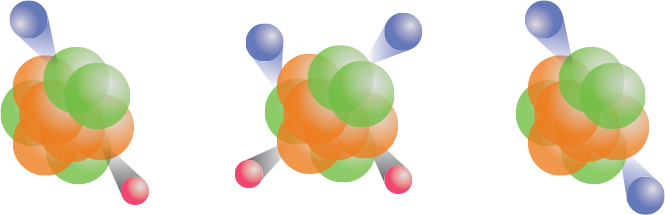
\includegraphics[width=0.6\textwidth]{bb-artist.png}};

    \node[align=center] at (-3.5,-1.9) {\scshape $\upbeta$ decay};
    \node[align=center] at ( 0.0,-1.9) {\scshape double-$\upbeta$ decay};
    \node[align=center] at ( 3.5,-1.9) {\scshape neutrinoless \\ \scshape double-$\upbeta$ decay};

    \node at (-4.3, 1.5) {$e^-$};
    \node at (-2.2,-1.1) {\footnotesize $\overline{\upnu}_e$};

    \node at (-1.2, 1.1) {$e^-$};
    \node at ( 1.4, 1.2) {$e^-$};
    \node at ( 1.3,-1.0) {\footnotesize $\overline{\upnu}_e$};
    \node at (-1.5,-0.9) {\footnotesize $\overline{\upnu}_e$};

    \node at ( 3.2, 1.5) {$e^-$};
    \node at ( 4.6,-1.2) {$e^-$};
  \end{tikzpicture}
\end{center}
In addition to being inevitably tied to the origins of the neutrino mass, neutrinoless
double-beta decay has a second critical consequence related to the fundamental laws of
Nature. One of the crucial conserved symmetries in the Standard Model concerns matter and
anti-matter: in all processes they must be produced, or destroyed, in the same amount.
The world we know, however, is evidently made of matter~---~and cosmological observations
seem to confirm that the rest of the universe looks very similar. How can it be that all
the balancing anti-matter predicted by the Standard Model is gone? The reader might have
realized now, after this preamble, that only matter (the two electrons) is produced in
neutrinoless double-beta decay. According to many theories, the existence of this process
might be enough to explain the asymmetry between matter and anti-matter produced in the
very early moments after the Big Bang. At this point, it is clear that the search for
neutrinoless double-beta decay is much more than a mere investigation of the properties of
a tiny fundamental particle. Its discovery would prove the existence of Majorana
neutrinos, physics beyond the Standard Model and perhaps shed light on the origins of our
universe.
\newpar
\blocktitle{\includegraphics[width=2.2cm]{gedet/bb-event.png}}
One of the candidate atomic nuclei for a discovery is the germanium isotope with mass
number 76. The experimental quest to discover neutrinoless double-beta decay in \gesix\
began more than fifty years ago, with the proposal by a group of researchers in
Milano~\cite{Fiorini1967}.  Germanium was already being used to build high-purity particle
detectors with excellent energy resolution, and the concept of incorporating the source in
the detector medium made the potential of this discovery channel immediately evident.
Since then, many experimental projects succeeded each other in developing the detector
technology and pushing forward the discovery sensitivity. None of them reported
unambiguous evidence for the existence of neutrinoless double-beta decay, and, in absence
of a signal, increasing lower limits on its half-life have been set. The \powtenyr{26}
threshold has been recently surpassed by the \gerda\ experiment, which is the subject of
this thesis work. \gerda\ was a \gesix\ experiment operating between \yr{2008} and
\yr{2019} at the Laboratori Nazionali del Gran Sasso, Italy. The core of the project was
an array of forty detectors submerged bare in liquid argon, which provided a passive and
active shield against external background, thanks to its scintillation properties. Thanks
to this and various other background mitigation techniques, \gerda\ has been operating in
background-free conditions (namely, less than a background count in the neutrinoless
double-beta decay search region in the entire measurement time) for the largest part of
its collected exposure. This achievement has successfully demonstrated the maturity of the
germanium technology as the base of a next-generation, tonne-scale experiment, which is
currently being prepared by the LEGEND collaboration.
\newpar
Searching for a signal in presence of a background is a common circumstance in a physics
experiment. Since the signal is hypothetical and possibly faint, the search for a signal
inevitably becomes a quest to reduce the background event rate in the search region as
much as possible. Several strategies are set up in \gerda\ both at the hardware level,
during design and construction, and at the software level, with data analysis routines.
Care is taken during the design phase not to expose the detectors to background sources
and to eventually mitigate their impact with passive or active shields. Materials for
setup items deployed in the vicinity of the detectors have been screened for the presence
of radioactive contaminants before deployment. Despite all these precautions, residual
backgrounds have to be expected and are indeed observed in the data. The task of the
background model is to identify the origin of these events by comparing the data collected
by the experiment to Monte Carlo simulations of radioactive contaminations in the setup.
The results are crucial to select the appropriate mitigation strategy when designing
future hardware upgrades or next-generation projects, and enhance the signal
sensitivity. Data selection algorithms can also benefit from an accurate knowledge of the
expected backgrounds.  Below in light blue is the energy spectrum of all events collected
by \gerda, together with the result of the background decomposition analysis, which is one
of the main subjects of this thesis.
\begin{center}
  \vspace{11pt}
  \includegraphics{plots/bkg/raw/combined-results-M1only.pdf}
\end{center}
The signature of neutrinoless double-beta decay is an event excess at the maximum energy
available in the process, indicated with a dashed line. The background model aims to give
an answer to the following questions: what kind of events dominate the background in the
region of interest? How many events from \b, \g\ and \a\ events are expected? What is
their interaction topology in the detectors? What are the sources and where are they
located?  Is the background uniform in the region, or peak-like structures have to be
expected?  What is the correct background model to be used in the neutrinoless double-beta
decay signal search? As it is evident from the picture above, an accurate description of
the full-energy spectrum is mandatory to extract solid predictions in the region of
interest.  The present thesis work aims to present and discuss the methodology developed
by the \gerda\ collaboration over the years and tries to give an answer to the questions
above.
\newpar
The development of a background model in double-beta decay experiments is, nonetheless,
not only devoted to the neutrinoless double-beta decay signal search. Along with that, the
potential of the two-neutrino decay as a precision test bench for the Standard Model and
theories beyond it must not be overlooked. An example of new-physics signal that
can be searched among the two-neutrino double-beta decay events is the so-called
neutrinoless double-beta decay with Majoron emission. In this hypothesized decay mode, two
electrons are emitted together with one or two additional bosonic particles that do not
interact with the detector medium. These processes would produce a deformation of the
two-neutrino double-beta decay energy spectrum (the olive green distribution in the figure
above) with respect to the Standard Model prediction.  One of the goals of the work
presented in the following chapters is to constrain the presence of the distortions that
could be associated with new-physics phenomena. Since backgrounds contribute to this
energy region as well, an accurate model is mandatory to extract the signal distribution
and precisely study the shape of the standard double-beta decay distribution. Data after
the liquid argon veto cut, which exploits the scintillation light emitted in liquid argon
in presence of background events, is analyzed for the first time.  To obtain theoretical
predictions on the background and signal distribution after the cut, a complete Monte
Carlo simulation of the veto system has been developed and tuned on calibration data.

The present thesis work is structured as follows. In \cref{chap:theory}, an overview of
the double-beta decay field is given, from the theoretical framework to the experimental
endeavors. The reader should then be equipped with a basic understanding of the theory
behind the standard two-neutrino mode as well as the new-physics modes and an overview of
the projects devoted to this search. In \cref{chap:gerda}, \gerda, the experiment on which
this work is based, is introduced with a description of the experimental apparatus and the
background reduction technologies that allow it to reach an unprecedentedly low background
in the region of interest for neutrinoless double-beta decay. At the end of the chapter
the final full-data set results on the search for the decay are presented and discussed.
The reader is introduced to the background model in \cref{chap:bkg:raw:ph2}, starting from
data before the high-level analysis cuts. The chapter starts with a description of the
analysis data set and continues with an overview of the Monte Carlo methods that are used
to generate the probability density functions for background sources. It follows an
illustration of the statistical framework in which the background decomposition is
performed and, finally, the results are discussed. The background model after the event
selection based on the scintillation light detected by the liquid argon veto system is
presented in \cref{chap:bkg:lar:ph2}. The Monte Carlo framework which has been developed
to simulate the propagation of optical photons in the experimental setup and obtain the
veto condition for synthetic events is described. The chapter flows straight to the final
\cref{chap:2nbb-ana}, which presents the analysis of the two-neutrino double-beta decay
distribution after the liquid argon veto cut, an improved estimate of the decay half-life
and constraints on new-physics processes. A final outlook on the work and appendices close
out the thesis.

\chapendgliph{}

% vim: tw=90
